\subsection{3I/ATLAS}\label{subsec:3I}

3I/ATLAS was discovered on 1 July 2025 by the ATLAS survey telescope at Río Hurtado, Chile \citep{seligman2025discoverypreliminarycharacterizationinterstellar}. It is the third interstellar object confirmed passing through the Solar System, after 1I/'Oumuamua (discovered 19 October 2017) and 2I/Borisov (discovered 29 August 2019). Given the rarity of the object and the excitement generated within the Rubin scientific community, we elected to test the ToO system on 3I/ATLAS. 

Many other science exposures of 3I/ATLAS have been obtained, as the object has been in the Rubin SV survey footprint for some time before its official identification. Here, we focus only on observations triggered by the ToO system.

\subsubsection{Night of July 12, 2025}

After consultation with the solar-system science unit, we devised an observing strategy for 3I/ATLAS that would maximize the probability of extracting color information, and determining its rotational period. 

\begin{figure}
    \centering
    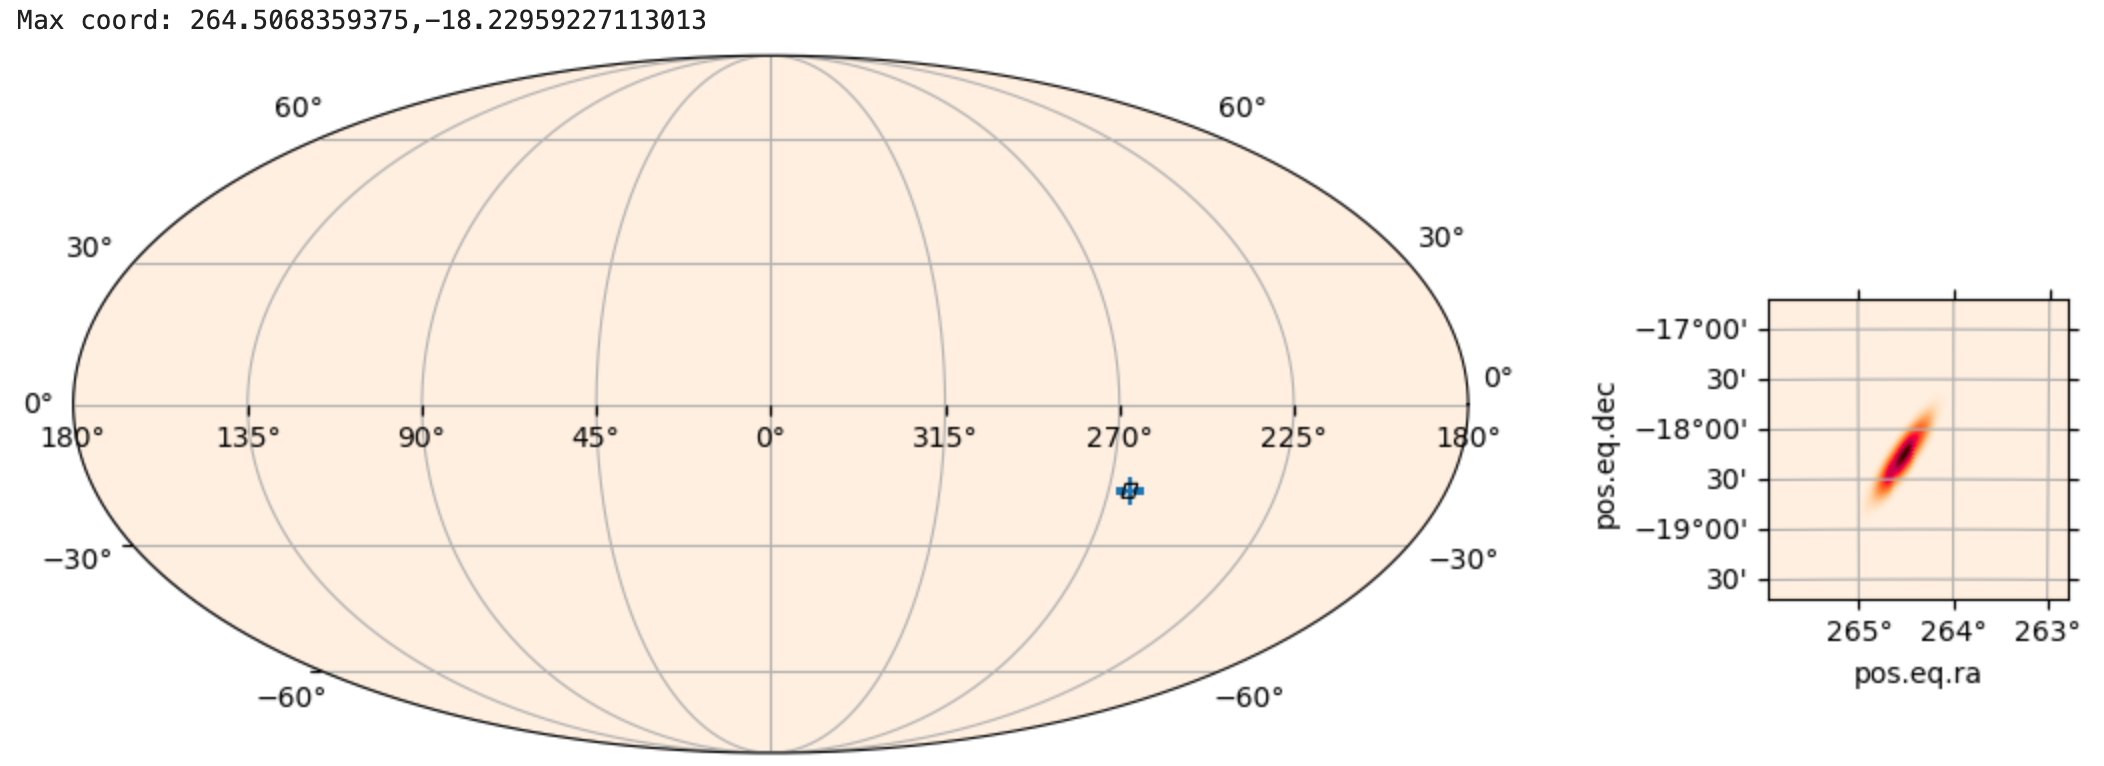
\includegraphics[width=1\linewidth]{figures/testsAndTriggers/3I_firstObs.png}
    \caption{The injected localization skymap for 3I/ATLAS ToO observations on the night of July 12, 2025.}
    \label{fig:3I_firstObs}
\end{figure}

The observing plan was as follows:

\begin{itemize}
    \item \textbf{Exposure times}: 30 second exposures.
    \item \textbf{Epochs}: One epoch at zero hours from alert receipt.
    \item \textbf{Visits}: Four visits for the single epoch.
    \item \textbf{Filters}: grizY for the single epoch.
    \item \textbf{Dithers}: Dither between exposures with a maximum of 0.01 degrees (36 arcseconds).
    \item \textbf{Safety masks}: The full suite of safety masks used by the SV surveys.
\end{itemize}

Since the localization area of 3I/ATLAS is extremely small ($<1\deg^2$), the injected alert localization was refined to fit within the nearest single $\texttt{NSIDE=32}$ flattened healpix pixel, which is the format utilized by the Rubin scheduler.

\begin{figure}
    \centering
    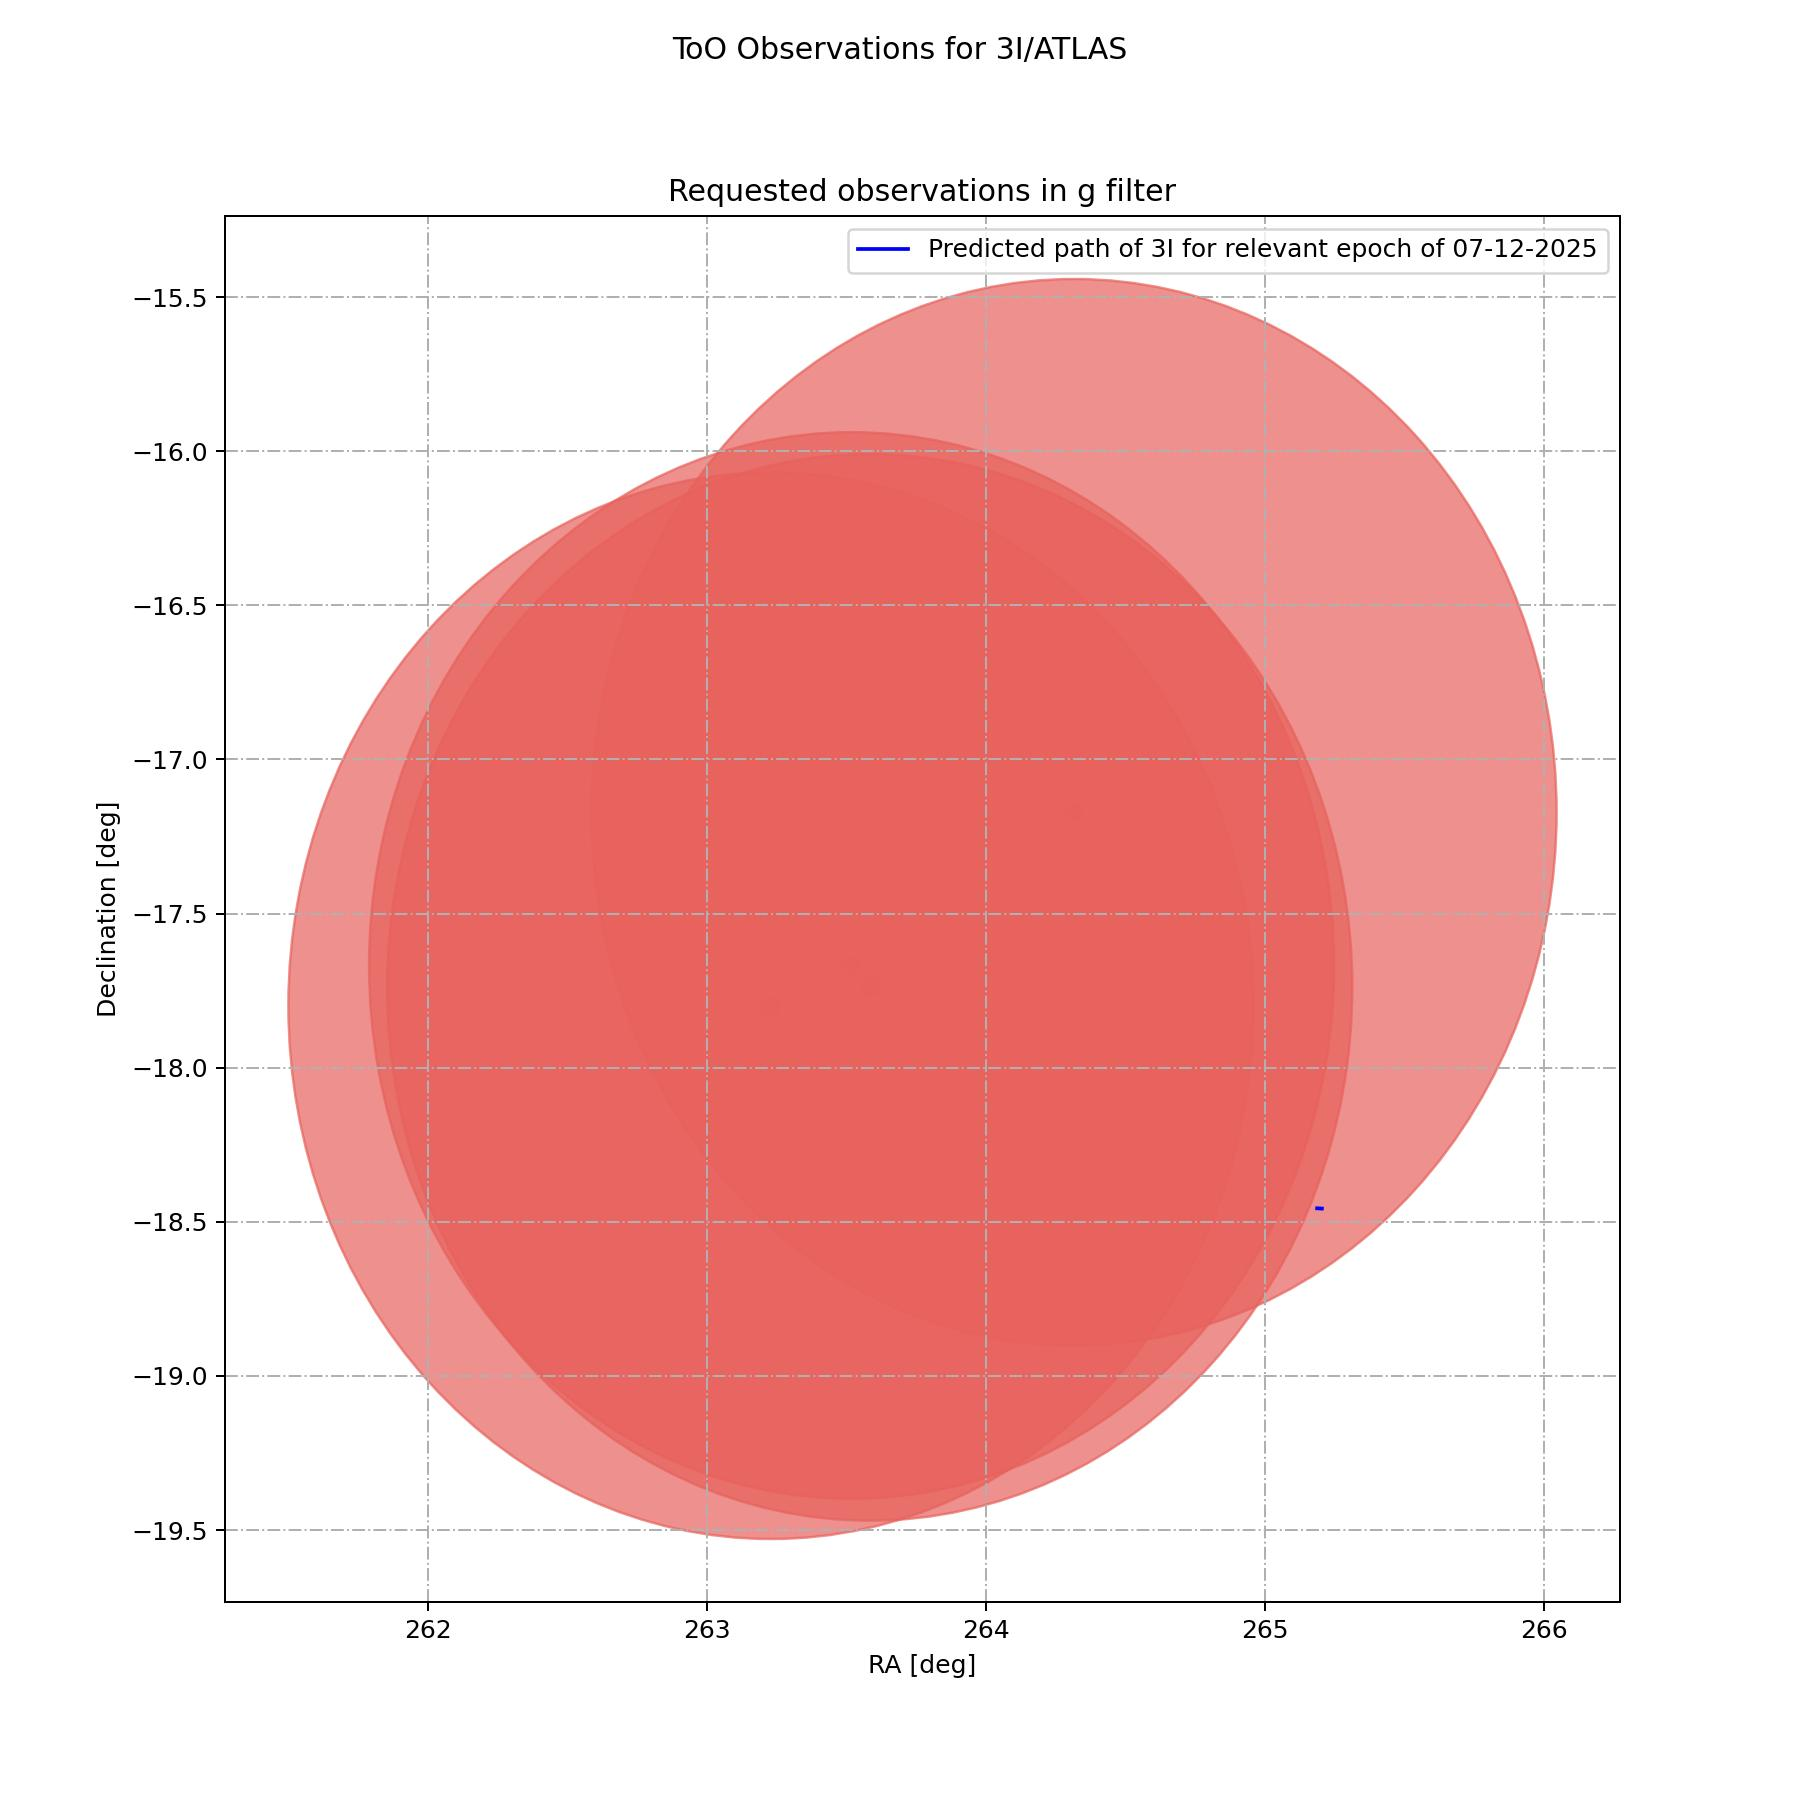
\includegraphics[width=0.5\linewidth]{figures/testsAndTriggers/3I_firstObs_filter_fromScheduler.png}
    \caption{The requested observations as generated from the scheduler configuration, with the predicted path of 3I/ATLAS during the observation epoch shown. Identical pointings were generated for i, r, z, and Y bands. Plotted circles are centered at the central pointing, with a radius reflective of the LSSTCam FOV.}
    \label{fig:3I_firstObs_filter}
\end{figure}

The alert was injected to the SCiMMA alert stream at 2:39:12 UTC, and received at the Rubin EFD. ToO observations of the 3I/ATLAS field began at 3:09:13 UTC shortly after the SV + ToO scheduler configuration was enabled, starting with observations in g band.

With four visits in the scheduler configuration, the expectation for observations was to have four visits per pointing in each filter, with the small dither between successive visits. Then, after the observations of a single filter were complete, the filter should change and proceed with observations in a different filter. 

The behavior of the scheduler during this ToO was subtly different. After observations in all five requested filters were obtained, the scheduler repeated the tilings an additional three times, totaling four cycles of observations in each filter. This repetitive cycle of four identical tilings appeared reflective of the configured visits.

Evaluation of the image processing for this event is ongoing, and has been impacted significantly by the USDF outage that began on July 7, 2025.

\begin{table}[ht]
\centering
\begin{tabular}{|l|p{10cm}|}
\hline
\textbf{Event} & \textbf{Timestamp / Details} \\
\hline
\textbf{Alert Injected} & 02:39:12 UTC \\
Received at Rubin EFD & Successfully received \\
\textbf{Alert processed by Scheduler CSC} & 03:08:09\\ \hline 
\textbf{Observations begin} & 03:09:13 \\
Cycles & 4 total cycles through all 5 filters \\
\textbf{End of ToO Observations} & 05:48:52 \\
\hline
\end{tabular}
\caption{Timeline of ToO observations for 3I/ATLAS on 2025-07-13, with times shown in UTC.}
\end{table}

The filter and visit behavior raises notable issues about this ToO observation from an operational perspective:

\begin{itemize}
    \item \textbf{Visit timing}: In the event of more than one visit in a single exposure epoch, the visits should be executed consecutively before changing filter. This minimizes the number of filter changes needed to complete the requested exposures, prolonging the lifetime of the filter exchanger hardware and maximizing survey efficiency.
    \item \textbf{Visit locations}: The area supplied to the Rubin scheduler for this ToO alert was one single healpixel of the $\texttt{NSIDE}=32$, closest to the target. Under the current tiling method, the boresight-pointing grid stays fixed, and can have multiple pointings inside a single $\texttt{NSIDE}=32$ pixel. Based on the repetitive behavior of exposures, there are currently two hypotheses for the pointing behavior.
    \begin{enumerate}
        \item The scheduler identified two pointings inside the healpix pixel, and imaged them with a dither in between.
        \item The scheduler identified four pointings inside the healpix pixel, and imaged them with a dither on the initial pointings 2-4.
    \end{enumerate}
\end{itemize}

\begin{figure}
    \centering
    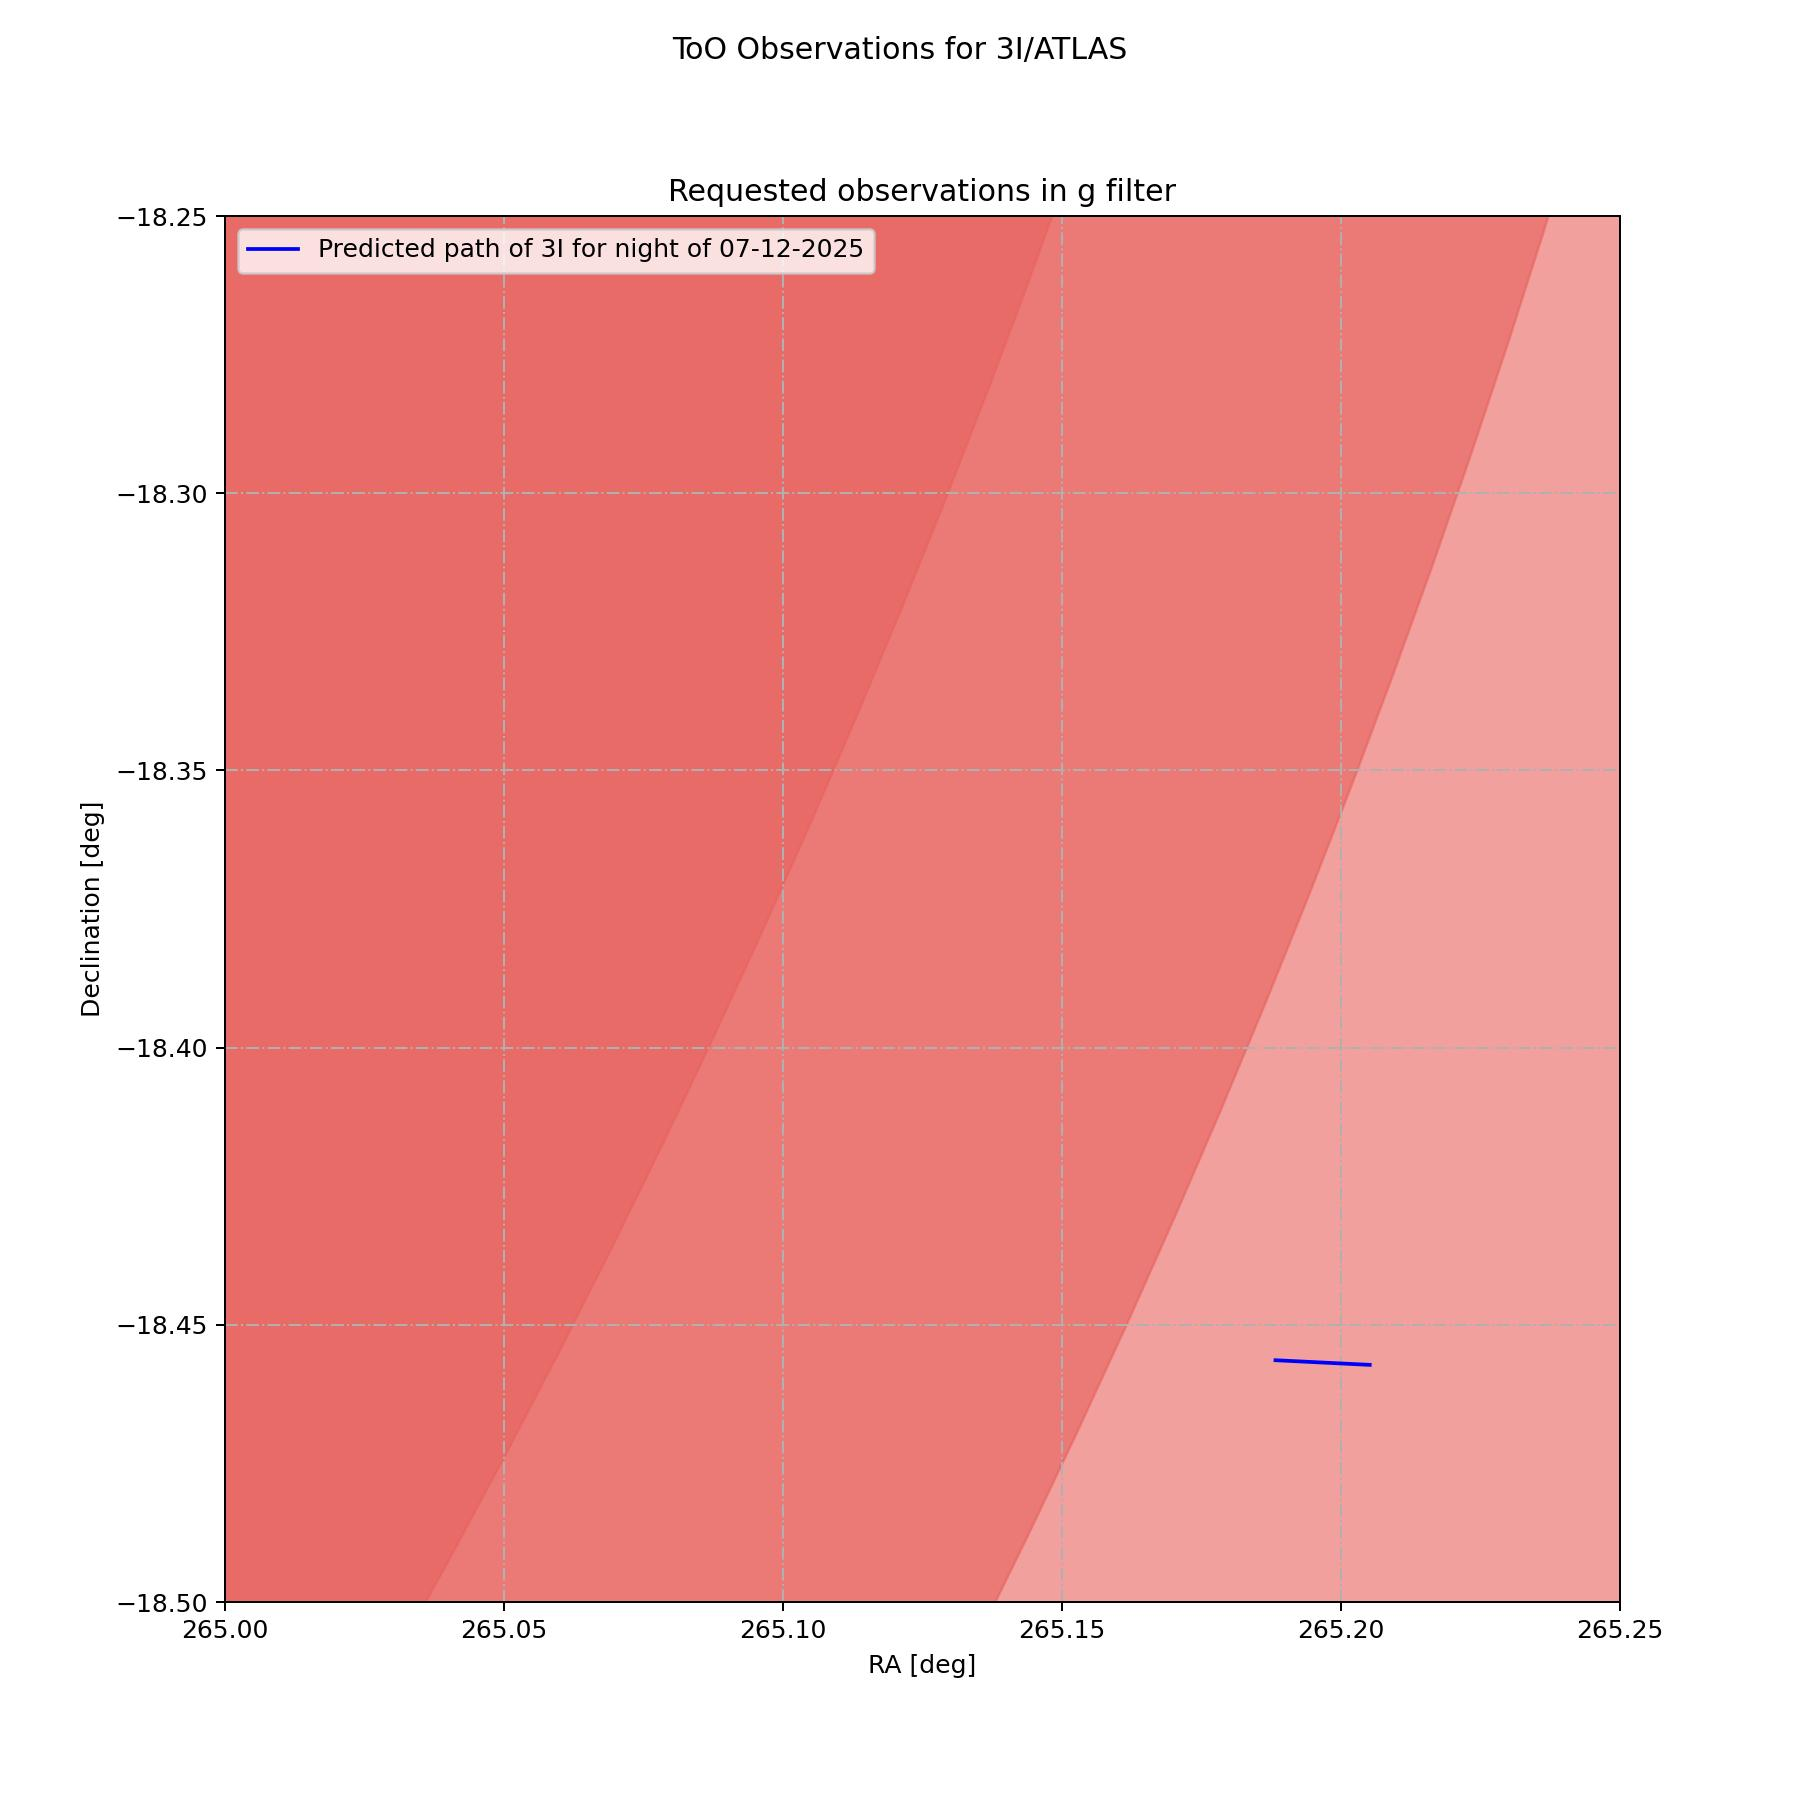
\includegraphics[width=0.5\linewidth]{figures/testsAndTriggers/3I_firstObs_filter_fromScheduler_inset.png}
    \caption{The same as figure \ref{fig:3I_firstObs_filter}, but a closeup of the predicted orbit. One exposure per band, per visit, captured 3I/ATLAS in its predicted orbit.}
    \label{fig:3I_firstObs_filter2}
\end{figure}

The pointing behavior needs further investigation to fully understand what is going on. However, immediate improvements can be made by defining a pointing grid for the ToO that has pointings centered on each healpix location. While this is \textbf{not} a final solution, this allows us to disentangle the root issue of visit timing vs. visit location behavior.


\subsection{GW event S250725j}\label{subsec:S250725j}

The gravitational wave event S250725j is a high-SNR binary black hole event that was observed by the LVK detector network at 04:09:58 UTC on 2025-07-25. S250725j was localized to a 90\% area of 18.6 $\deg^2$, meeting the alert quality criteria for a BBH event from \cite{RubinToO2024}.

After discussion within the Rubin-commissioning ToO advisory board, we elected to trigger a ToO on S250725j.

\subsubsection{Night of July 28, 2025}

The observing plan was as follows:

\begin{itemize}
    \item \textbf{Exposure times}: 30 second exposures.
    \item \textbf{Epochs}: Epoch spacing as requested in \cite{RubinToO2024} (see below).
    \item \textbf{Visits}: one visit per epoch.
    \item \textbf{Filters}: u-g-r requested, u-g-i observed (see below).
    \item \textbf{Dithers}: Dither between exposures with a maximum of 0.01 degrees (36 arcseconds).
    \item \textbf{Safety masks}: The complete suite of safety masks used by the SV surveys.
\end{itemize}

\begin{figure}[b!]
    \centering
    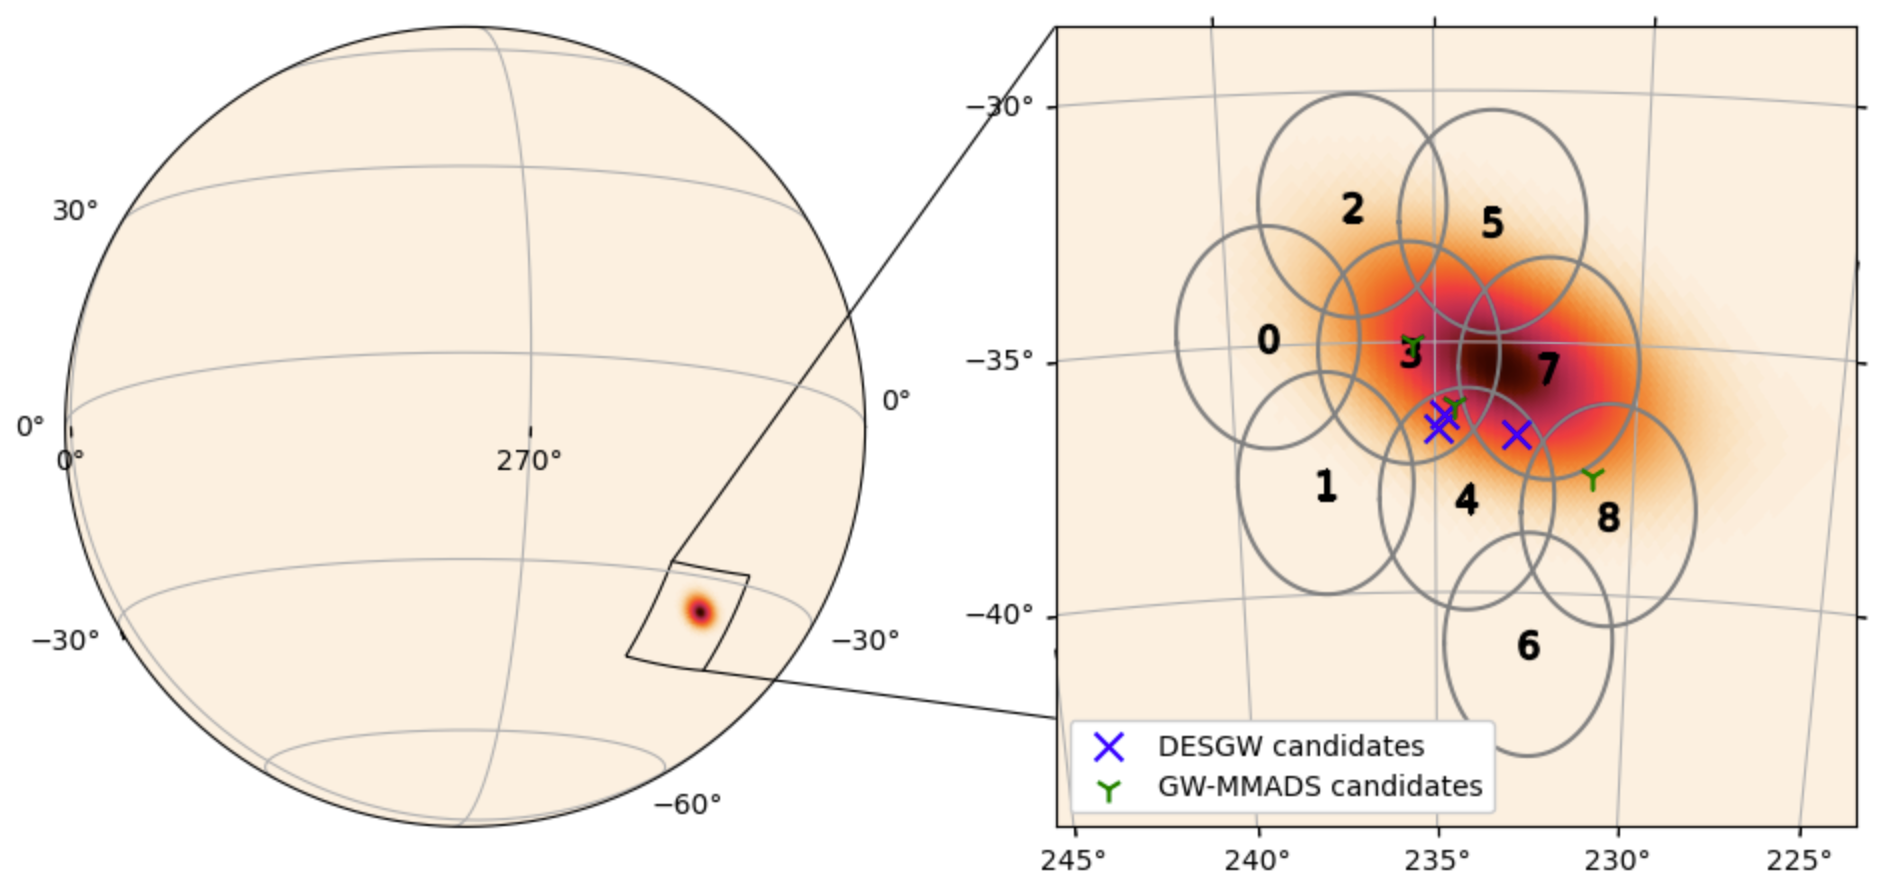
\includegraphics[width=\linewidth]{figures/testsAndTriggers/25j_skymap.png}
    \caption{Left: The skymap of S250725j, showing the localization area concentrated near $(234º, -35º)$. Right: The pointings acquired as part of the 2025-07-28 observations shown in grey circles. The area covered by the Rubin pointings covers 94\% of the LVK localization probability. Candidates reported by other observing teams using DECam are shown overplotted on the skymap.}
    \label{fig:25j-skymap}
\end{figure}

Epoch spacing for this ToO was planned around log-spacing observations over nights, resulting in observations on nights 1-3-8-10-39 after the alert is received. In practice, the observations from the night of 2025-07-28 were the only observations obtained due to a combination of weather constraints and other commissioning activities.

The filter request for a binary-black hole merger of this distance and type is u-g-r bands. Due to an engineering problem with the FCS of LSSTCam, the g band was not available. As a result, we set the observing strategy to observe in u-r-i bands.

The alert packet was submitted to the ToO alert stream at 02:16:22.407 UTC, and received at the Rubin EFD at 02:16:25 UTC, approximately 3 seconds later.

Conditions on the night of observing were nominal. We reached a median depth of 24.1 mag in r band, 23.8 mag in the i band, and 23.6 in u band. An issue in the Scheduler CSC caused the field to be observed two times, mimicking previous ToO tests where the Scheduler CSC continued observing the field of a ToO until the scheduler configuration was disabled.


\subsubsection{Pointing efficiency}

This ToO is the first test on-sky of a ToO area that is larger than a single Rubin pointing. Therefore, this event provides a unique opportunity to evaluate the efficiency of covering a ToO area to completion. For all GW ToO events, the relevant area that needs to be covered is the 90\% area. A detailed analysis of point efficiency for this event can be found in the \href{https://github.com/lsst-sitcom/ToO-analysis-tools/blob/ef84da607cad62606d489eb61ee7aa4e61063e4c/notebooks/PointingEfficiency.ipynb}{\texttt{ToO-analysis-tools}} github repository.

\begin{figure}
    \centering
    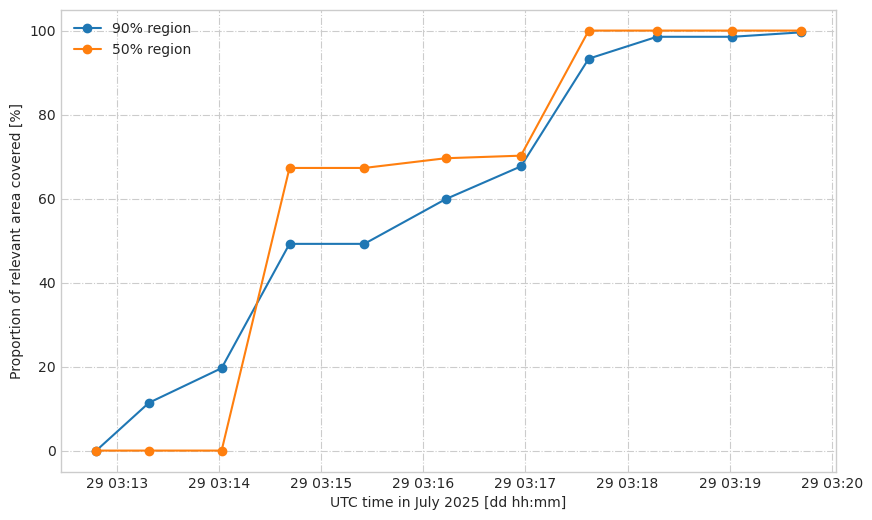
\includegraphics[width=\linewidth]{figures/testsAndTriggers/efficiencyFig.png}
    \caption{The efficiency of covering the area of S250725j, represented as a proportion of the 50\% and 90\% localization areas.}
    \label{fig:pointingEfficiencyFig}
\end{figure}

For each pass in each filter, 100\% of the 50\% probability region was covered, and 99.576\% of the 90\% region was covered. Additionally, the 50\% region was covered at a rate of $1.64 \deg^2$/min, and the 90\% region was covered at a rate of 4 $\deg^2/$min.

\subsubsection{Image processing and candidate vetting}

\begin{figure}[b]
    \centering
    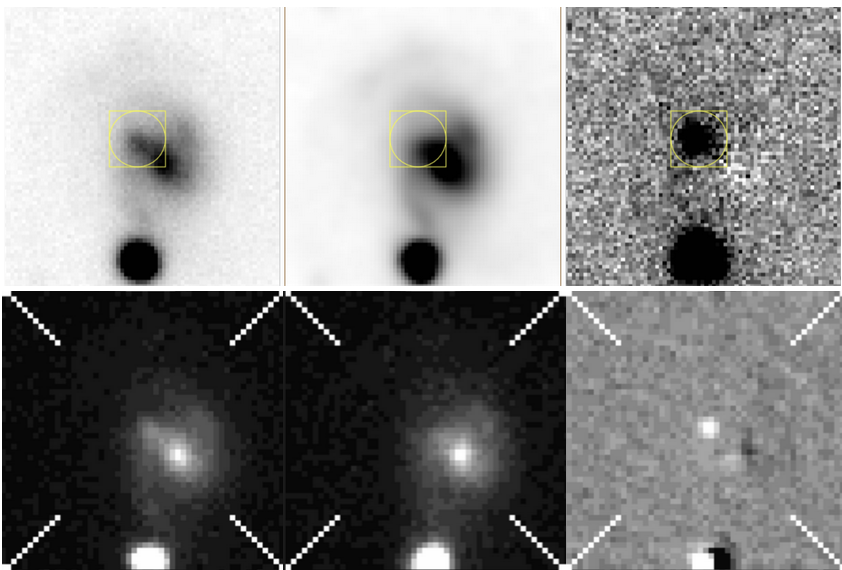
\includegraphics[width=\linewidth]{figures/testsAndTriggers/candidateComparison_25j.png}
    \caption{AT2025sib, one of the four reported Rubin candidates in GCN 41595, as viewed by LSSTCam and DECam, each with a field of view of ~14" on each edge. The top row of images are from Rubin Observatory, the bottom row of images were taken with DECam. Search (left), template (center), and difference (right) images. The template images for Rubin difference imaging are from DES DR2 co-additions for this region of the sky.}
    \label{fig:25j_candidateComparison}
\end{figure}

To process and analyze the observations from this event, we used the bespoke image processing pipeline as described in section \ref{subsec:systemTests verification}. For this region of the sky, template level coadds from DES DR2 were available.

The location of this GW event is nearby the galactic plane, and therefore a crowded field. Proximity to the galactic plane causes well known problems with the WCS solution. The issues with the WCS solution in search images propagates to the difference images, resulting in many bad subtractions, dipoles, and other artifacts in the difference images.

% Maybe add an image of the bad wcs fits here?

After processing the relevant visits through the bespoke image processing pipeline, we applied a minimal set of flags to remove visits that have dipoles, cosmic rays, and other artifacts. Despite this quality cut, we identified $\sim25$k DIA candidates per visit, which far exceeds the ability of human vetting capabilities.

After assessing the excess of candidates from the bespoke image processing pipeline, the analysis group pivoted to review of transient candidates reported by other teams using DECam (see figure \ref{fig:25j_candidateComparison}). The results of the inspection of DECam candidates were reported in GCN 41595 \citep{MacBride_Anand_Howard_2025}.